\documentclass[conference]{IEEEtran}
\IEEEoverridecommandlockouts
\usepackage{cite}
\usepackage{amsmath,amssymb,amsfonts}
\usepackage{graphicx}
\usepackage{textcomp}
\usepackage{xcolor}
\usepackage{float}
\usepackage{booktabs}
\usepackage{array}

\def\BibTeX{{\rm B\kern-.05em{\sc i\kern-.025em b}\kern-.08em
    T\kern-.1667em\lower.7ex\hbox{E}\kern-.125emX}}

\begin{document}

\title{End-to-End Semantic Perception and Geometry-Based Adaptive Control for Edge Autonomous Racing\\}

\author{
    \IEEEauthorblockN{Quang Nhan Hoang}
    \IEEEauthorblockA{\textit{FPT University} \\
        Ho Chi Minh City, Vietnam}
    \and
    \IEEEauthorblockN{Duc Nguyen Huu Dang}
    \IEEEauthorblockA{\textit{FPT University} \\
        Ho Chi Minh City, Vietnam}
    \and
    \IEEEauthorblockN{Thien Vuong Kim Hoang}
    \IEEEauthorblockA{\textit{FPT University} \\
        Ho Chi Minh City, Vietnam}
}

\maketitle

\begin{abstract}
    Deploying deep learning-driven autonomous driving systems on resource-constrained embedded edge platforms, such as the NVIDIA Jetson Nano, presents severe computational and latency challenges. This paper presents a robust, edge-optimized autonomous driving framework designed specifically for the Jetson AI Racer Challenge 2026. We propose a hybrid architecture that integrates a customized, highly pruned YOLO26 semantic segmentation network, deterministic geometry-driven path planning, a hierarchical state-aware adaptive proportional-integral-derivative (PID) controller, and an automated green-marker start gate. The perception pipeline predicts dense masks for drivable road, center divider, and forbidden shoulder regions at $224 \times 224$ resolution, achieving $>25$ FPS inference via TensorRT FP16 optimization and graph rewrites. Mathematical polynomial regression and multi-row candidate extraction dynamically generate collision-free navigation trajectories, while the adaptive controller orchestrates latency-aware maneuvers, including Electronic Speed Controller (ESC)-safe reverse recovery and road-reacquisition. Experimental profiling demonstrates strict adherence to the competition's 300 ms end-to-end latency constraint, providing exceptional track adherence and dynamic recovery on physical scale tracks.
\end{abstract}

\begin{IEEEkeywords}
    Autonomous Racing, Semantic Segmentation, Edge Computing, TensorRT, Path Planning, Adaptive Control, Jetson Nano.
\end{IEEEkeywords}

\section{Introduction / Motivation}
The rapid evolution of artificial intelligence and deep neural networks has substantially enhanced the capabilities of autonomous vehicles (AVs) in perception, localization, and motion planning. However, migrating state-of-the-art vision models from server-class GPUs to power- and resource-constrained edge platforms remains an open engineering challenge. The Jetson AI Racer Challenge 2026 presents an exacting benchmarking scenario where miniature $1/10$-scale autonomous vehicles must negotiate complex circuit geometries (Speed Track) and rule-based urban intersections (Smart City) under strict real-time constraints.

Operating on the NVIDIA Jetson Nano (equipped with a 128-core Maxwell GPU and 4 GB shared LPDDR4 memory) introduces acute computational, thermal, and memory bottlenecks \cite{ref1, ref2}. Conventional edge AV pipelines typically combine disparate heuristics: sparse edge detection (e.g., Canny filters, Hough transforms) for lane extraction and bounding-box object detectors for obstacles \cite{ref3}. In practice, such systems degrade rapidly under motion blur, variable ambient illumination, non-uniform track textures, and partial occlusions.

The core motivation of this research is to architect a unified, hybrid perception-and-control framework that maximizes inference throughput and algorithmic reliability without sacrificing fine-grained spatial awareness. We demonstrate that by combining dense, low-resolution semantic segmentation with deterministic mathematical trajectory modeling and a finite-state machine (FSM) adaptive controller, an embedded edge racer can achieve high-speed stability, robust obstacle avoidance, and autonomous off-track recovery within strict computational budgets.

\section{Problem Statement \& Research Questions}
The competition rules stipulate that vehicles must complete race tracks autonomously, adhere strictly to lane boundaries, pass mandatory sequential checkpoints, avoid dynamic obstacles, and maintain a total pipeline latency below 300 ms. This gives rise to three fundamental research questions:
\begin{enumerate}
    \item \textbf{Edge Perception Efficiency}: How can pixel-level dense semantic segmentation be executed on a Jetson Nano at $>20$ FPS while maintaining high segmentation fidelity across road boundaries, center dividers, and forbidden zones?
    \item \textbf{Robust Trajectory Extraction}: How can the navigation trajectory be mathematically formulated to isolate true path features from noisy edge masks and dynamic obstacle occlusions?
    \item \textbf{Dynamic Control Stability \& Actuator Safety}: How to design a multi-state control architecture that transitions seamlessly between high-speed racing, curve deceleration, and multi-stage reverse recovery while respecting the physical voltage and ESC switching limits?
\end{enumerate}

\section{Related Work}
Autonomous driving architectures on embedded systems have progressed through several distinct paradigms. Early methodologies relied heavily on classical computer vision pipelines, including inverse perspective mapping (IPM), color thresholding in HSV/LAB spaces, and sliding-window polynomial fitting \cite{ref4}. While computationally frugal, these techniques are brittle against specular reflections, shadows, and varying asphalt colors.

The advent of Convolutional Neural Networks (CNNs) brought real-time object detection models like YOLO to edge devices \cite{ref5, ref6}. While bounding boxes effectively identify localized obstacles and traffic signs, they lack topological road awareness, which is essential for steering along curved boundaries.

Conversely, dense semantic segmentation networks (such as U-Net, PSPNet, and DeepLab) provide comprehensive pixel-level labeling but incur prohibitive FLOPs and memory footprints that lead to out-of-memory (OOM) errors or low frame rates ($<5$ FPS) on edge hardware \cite{ref7, ref8}. Recent works in autonomous racing have explored hybrid paradigms where lightweight backbones are combined with mathematical curves or spline fits \cite{ref9, ref10}. Building on this foundation, our work presents an end-to-end engineered system featuring custom ONNX graph optimization, TensorRT FP16 deployment, geometric candidate evaluation, and an ESC-aware FSM controller.

\section{Proposed Method}
The complete system architecture, illustrated in Fig. \ref{fig:arch}, comprises four deeply integrated subsystems: (i) Optimized Semantic Perception, (ii) Deterministic Geometry Path Planning, (iii) Hierarchical State-Aware Adaptive Control, and (iv) Automated Start Gate Interlocking.

\begin{figure}[htbp]
    \centerline{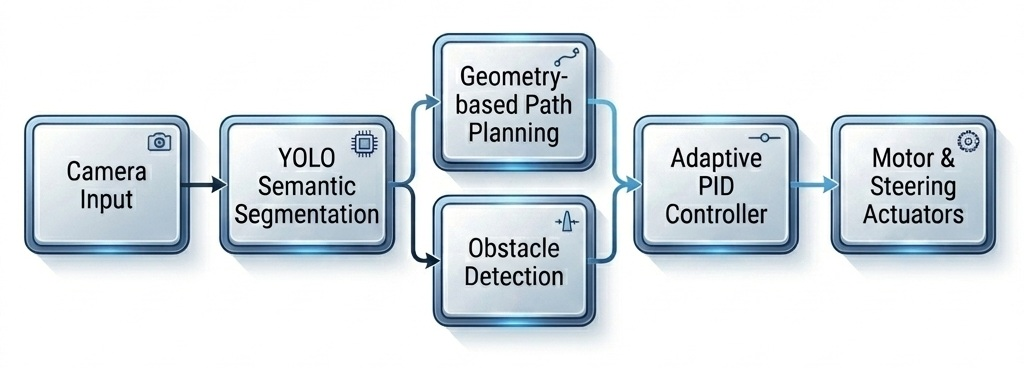
\includegraphics[width=0.48\textwidth]{fig1_arch.jpg}}
    \caption{Overall system architecture demonstrating the data flow from the CSI Camera input to TensorRT inference, geometry planning, FSM controller, and motor actuators.}
    \label{fig:arch}
\end{figure}

\subsection{Semantic Perception \& TensorRT Graph Optimization}
The perception subsystem utilizes a specialized, compact YOLO26 semantic segmentation network trained on track-specific datasets. To satisfy embedded latency constraints, input frames captured from the onboard wide-angle CSI camera are downsampled to $224 \times 224$ pixels. The network outputs dense semantic masks across four mutually exclusive classes: $\mathcal{C} \in \{\text{Background } (0), \text{Road } (1), \text{Divider } (2), \text{Forbidden } (3)\}$.

\begin{figure}[htbp]
    \centering
    \begin{tabular}{cc}
        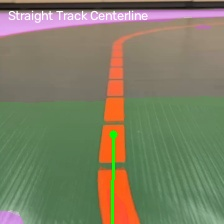
\includegraphics[width=0.23\textwidth]{fig2_seg_1.jpg} & 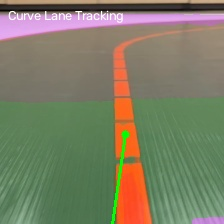
\includegraphics[width=0.23\textwidth]{fig2_seg_2.jpg} \\
        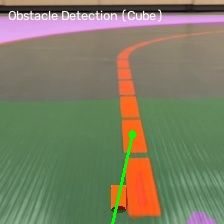
\includegraphics[width=0.23\textwidth]{fig2_seg_3.jpg} & 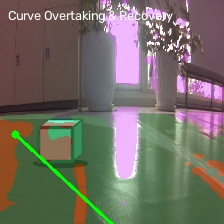
\includegraphics[width=0.23\textwidth]{fig2_seg_4.jpg}
    \end{tabular}
    \caption{FPV semantic segmentation predictions across challenging track conditions, showing clear classification of drivable road, center divider, and forbidden white boundaries.}
    \label{fig:seg}
\end{figure}

\subsubsection{ONNX Graph Surgery and TensorRT Compilation}
Exporting modern transformer-augmented segmentation heads directly to TensorRT on NVIDIA JetPack 4.6 (TensorRT 8.x) exposes compatibility barriers. Specifically:
\begin{itemize}
    \item \textbf{Static Split Replacement}: The attention layers in YOLO26 generate an opset-13 Split node with uneven split partition sizes (32, 32, 64) defined as constant inputs. TensorRT 8.x fails to parse dynamic constant split parameters correctly. We implement custom ONNX graph surgery that rewrites these nodes into static, deterministic Slice operations with explicit starts, ends, axes, and steps initializers.
    \item \textbf{Type Cast Sanitization}: TensorRT 8.x rejects UINT8 output casts from ArgMax operations. The export pipeline systematically replaces all UINT8 cast targets with INT32 data types.
\end{itemize}
The sanitized graph is compiled into a serialized FP16 TensorRT engine with a fixed workspace budget of 512 MiB:
\begin{equation}
    \mathcal{E} = \text{BuildEngine}(\mathcal{M}_{ONNX}, \text{FP16}=\text{True}, \mathcal{W}_{max}=512\,\text{MiB})
\end{equation}
A pre-flight warmup routine passes a blank dummy tensor through the engine prior to camera initialization, eliminating first-frame JIT latency spikes.

\subsubsection{Spatial ROI Slicing and Temporal Filtering}
To assess immediate lateral boundary hazards, the forbidden mask $M_{forbidden}$ is partitioned into three regions of interest (ROIs):
\begin{align}
    F_L       & = \frac{1}{|ROI_L|} \sum_{(x,y) \in ROI_L} M_{forbidden}(x,y)             \\
    F_R       & = \frac{1}{|ROI_R|} \sum_{(x,y) \in ROI_R} M_{forbidden}(x,y)             \\
    F_{front} & = \frac{1}{|ROI_{front}|} \sum_{(x,y) \in ROI_{front}} M_{forbidden}(x,y)
\end{align}
where $ROI_{front} = \{(x,y) \mid y \ge 0.62 h,\, 0.30 w \le x \le 0.70 w\}$.

Furthermore, a lower-horizon safe-road clearance metric evaluates the drivable road support in the left vs. right half-spaces below the lookahead horizon ($y \ge y_{look}$). If $\max(N_{left}, N_{right}) \ge N_{min\_hint}$, the module generates a deterministic escape heading hint:
\begin{equation}
    \delta_{escape} = \begin{cases}
        +1.0, & \text{if } N_{right} > N_{left} \\
        -1.0, & \text{if } N_{left} > N_{right} \\
        0.0,  & \text{otherwise}
    \end{cases}
\end{equation}
To prevent frame-to-frame jitter, detection confidence $C$ is smoothed via an Exponential Moving Average (EMA):
\begin{equation}
    C_t = \alpha_c C_{curr} + (1 - \alpha_c) C_{t-1}, \quad \alpha_c = 0.35
\end{equation}
Additionally, a rate-of-change limiter clamps consecutive target offsets: $|\Delta x_{target}| \le 28$ pixels per frame.

\subsection{Geometry-Based Target Trajectory Extraction}
The geometry planning module converts raw segmentation bitmasks into a continuous mathematical trajectory.

\subsubsection{Connected Component Selection}
Raw divider predictions can exhibit disconnected noise or distant background artifacts. We identify connected components using 8-connectivity and evaluate a composite tracking score $S$:
\begin{equation}
    S = 2.0 \cdot y_{norm} + c_{cov} + \min\left(\frac{A}{300}, 1.0\right) - 2.2 \cdot p_{center}
\end{equation}
where $y_{norm} = (y_{min} + bh)/h$ represents the normalized bottom position, $c_{cov} = bh/h$ is the vertical coverage ratio, $A$ is the component pixel area, and $p_{center} = |x_{near} - w/2|/w$ penalizes lateral deviation from the vehicle's optical center. To minimize computational latency ($O(\text{labels} \times hw)$), $x_{near}$ is computed solely on the lower 30\% bounding box slice: $y \in [y_{min} + 0.7 bh, y_{min} + bh]$.

\subsubsection{Equalized Polynomial Fitting}
From the selected divider component, row-wise horizontal centroids $\bar{x}(y)$ are extracted across all valid rows where row pixel counts exceed threshold $\tau_{row}$:
\begin{equation}
    \bar{x}(y) = \frac{\sum_{x} x \cdot M(x,y)}{\sum_{x} M(x,y)}, \quad \forall y \ge y_{top}
\end{equation}
Equalizing the row weights ensures that thick segmentations near the image bottom do not disproportionately bias the curve. A second-degree polynomial regression is performed:
\begin{equation}
    x(y) = a y^2 + b y + c
\end{equation}
From this curve, we sample the lookahead target point $x_{target} = x(y_{look})$ at $y_{look} = 0.60 h$ and the near-field base point $x_{near} = x(y_{near})$ at $y_{near} = 0.93 h$. The heading error $\theta_{err}$ and lane curvature $\kappa$ are computed as:
\begin{align}
    \theta_{err} & = \text{clip}\left(\frac{x_{target} - x_{near}}{\max(1.0, y_{near} - y_{look})}, \right. \nonumber \\
                 & \quad\quad\quad \left. -1.0, 1.0\vphantom{\frac{1}{1}}\right)                                      \\
    \kappa       & = \text{clip}(|2a| \cdot h, 0.0, 1.0)
\end{align}
The geometric estimate confidence $C_{geom}$ is formulated with a multi-line split to maintain strict column boundaries:
\begin{equation}
    \begin{split}
        C_{geom} = \text{clip}\left(0.75 \cdot \frac{N_{active\_rows}}{h - y_{top}} \right. & \\
        + \left. 0.25 \cdot \min\left(1.0, \frac{A_{roi}}{350}\right), 0.0, 1.0\right) &
    \end{split}
\end{equation}

\subsubsection{Dynamic Road Corridor and Obstacle Evaluation}
When an obstacle or forbidden barrier obstructs the center corridor ($W_{safe} = [x_{target} - w_{veh}, x_{target} + w_{veh}]$), the planner evaluates navigable corridors in the road mask.
Morphological closing ($\text{kernel } 5 \times 5$) fuses road and divider masks into a composite traversable space, while forbidden and obstacle regions are dilated by the full vehicle width ($2 w_{veh} + 1$). The algorithm searches horizontal candidate spans (row candidates) that satisfy complete vehicle-width clearance ($2 w_{veh} + 1$) simultaneously at both $y_{look}$ and $y_{near}$ within a maximum drift constraint $|x_{look} - x_{near}| \le 5 w_{veh}$, yielding a collision-free avoidance target.

\subsection{Adaptive PID Control and Actuator Maneuver Logic}
The control subsystem translates geometric path parameters into low-level steering ($\delta$) and throttle ($\tau$) commands.

\subsubsection{Augmented Lateral Tracking}
The lateral error is normalized relative to the camera center: $e = (x_{target} - w/2) / (w/2)$. To eliminate steady-state offset on banked or curved turns while providing anticipatory damping, we augment the standard PID formulation with a heading feedforward term:
\begin{equation}
    \delta_{raw} = K_p e + K_i \int_{0}^{t} e \, dt + K_d \frac{de}{dt} + K_h \theta_{err}
\end{equation}
Anti-windup clamping restricts the integral term: $\int e \, dt \in [-0.5, 0.5]$. High-frequency servo chatter is suppressed by a first-order low-pass filter followed by a slew-rate limiter:
\begin{align}
    \delta_{filt} & = \alpha_s \delta_{raw} + (1 - \alpha_s) \delta_{last\_raw}, \quad \alpha_s = 0.85                    \\
    \delta_t      & = \delta_{t-1} + \text{clip}(\delta_{filt} - \delta_{t-1}, -\Delta \delta_{max}, \Delta \delta_{max})
\end{align}
where $\Delta \delta_{max} = 0.45$ per control cycle.

\subsubsection{Longitudinal Ramping \& Voltage Droop Prevention}
Abrupt motor acceleration draws large instantaneous currents that can induce battery voltage sag, triggering an involuntary reset of the Jetson Nano. To prevent this, throttle commands are governed by an asymmetric rate-limiter:
\begin{equation}
    \tau_t = \tau_{t-1} + \text{clip}(\tau_{target} - \tau_{t-1}, -\Delta_{down}, \Delta_{up})
\end{equation}
with acceleration step $\Delta_{up} = 0.25$ and deceleration step $\Delta_{down} = 0.35$.

\subsubsection{Hierarchical Finite State Machine (FSM)}
The controller executes a state machine with latched safety overrides:
\begin{itemize}
    \item \textbf{Lane Lock Acquisition (Wait Lane Lock)}: The vehicle remains stationary until perception confirms valid lane locks for $N_{confirm} \ge 3$ consecutive frames with $C \ge 0.55$.
    \item \textbf{Nominal Tracking (Follow)}: Operates closed-loop PID lateral tracking and throttle control.
    \item \textbf{Dropout Tolerance (Slow Lane Dropout)}: If lane lock is momentarily dropped ($\le 3$ frames), the controller maintains forward momentum at cruise throttle to navigate through sensor gaps.
    \item \textbf{Road Reacquisition (Reacquire Road)}: If lost frames exceed $N_{lost} > 3$, the controller zeroes the integral term, applies escape steering $\delta_{escape}$, and searches for drivable road.
    \item \textbf{ESC-Safe Reverse Recovery (White Neutral $\rightarrow$ White Reverse $\rightarrow$ White Correct)}: When $F_{front} \ge 0.58$ persists for 2 frames, direct forward motion is unsafe. Crucially, physical Electronic Speed Controllers (ESCs) require a neutral zero-throttle pulse before engaging reverse torque. The FSM injects a 120 ms neutral state ($\tau = 0.0$), engages reverse gear ($\tau = -0.11$) with maximum counter-steering away from the boundary for 350 ms, and completes the maneuver with a forward correction pulse ($\tau > 0$) toward the center divider.
    \item \textbf{Side Boundary Correction (White Correct)}: If $F_L \ge 0.12$ or $F_R \ge 0.12$ exceeds the opposite side by margin $\Delta F \ge 0.04$, the controller applies proactive lateral bias without stopping.
\end{itemize}

\subsection{Competition Start Gate \& Motor Interlocking}
To comply with competition regulations, an automated start gate subsystem processes camera frames prior to race authorization.
\begin{itemize}
    \item \textbf{Color Segmentation}: Images are converted to HSV color space and segmented for green wavelengths: $H \in [38, 88], S \in [100, 255], V \in [120, 255]$.
    \item \textbf{Morphological Filtering \& Contour Geometry}: Morphological opening and closing kernels ($5 \times 5$) remove speckle noise. Contours are filtered based on circularity $\mathcal{C} = \frac{4\pi A}{P^2} \ge 0.82$ and bounding area ratio $A/A_{img} \in [0.002, 0.20]$.
    \item \textbf{Debounced Latch}: Detection must persist for $N \ge 3$ consecutive frames before authorizing motor start. Motor actuation is governed by a strict triple interlock:
          \begin{equation}
              \text{Motor\_Enable} = \text{Armed} \land (\neg \text{Ready} \lor \text{Authorized}) \land \text{SafeState}
          \end{equation}
\end{itemize}

\begin{table}[htbp]
    \caption{System Parameters and Controller Hyperparameters}
    \label{tab:params}
    \centering
    \resizebox{\columnwidth}{!}{%
        \begin{tabular}{llr}
            \toprule
            \textbf{Subsystem} & \textbf{Parameter / Configuration}             & \textbf{Value}   \\
            \midrule
            Perception         & Input Image Resolution ($H \times W$)          & $224 \times 224$ \\
                               & Segmentation Model Backbone                    & YOLO26n-sem      \\
                               & Quantization Precision                         & TensorRT FP16    \\
                               & Confidence Threshold                           & 0.35             \\
                               & Confidence EMA Factor ($\alpha_c$)             & 0.35             \\
            \midrule
            Geometry           & Lookahead Ratio ($y_{look}$)                   & 0.60 ($134$ px)  \\
                               & Near-Field Base Ratio ($y_{near}$)             & 0.93 ($208$ px)  \\
                               & ROI Top Ratio ($y_{top}$)                      & 0.45 ($100$ px)  \\
                               & Vehicle Half-Width ($w_{veh}$)                 & 13 px            \\
                               & Minimum Row Mask Pixels                        & 35 px            \\
            \midrule
            Controller         & Proportional Gain ($K_p$)                      & 0.92             \\
                               & Integral Gain ($K_i$)                          & 0.02             \\
                               & Derivative Gain ($K_d$)                        & 0.10             \\
                               & Heading Gain ($K_h$)                           & 0.42             \\
                               & Max Steering Slew Step ($\Delta \delta_{max}$) & 0.45 / frame     \\
                               & Throttle Acceleration Step ($\Delta_{up}$)     & 0.25 / frame     \\
                               & Throttle Deceleration Step ($\Delta_{down}$)   & 0.35 / frame     \\
                               & Nominal Cruise Throttle ($\tau_{cruise}$)      & 0.85 (85\%)      \\
                               & Maximum Throttle ($\tau_{max}$)                & 1.00 (100\%)     \\
            \midrule
            Safety             & Front Forbidden Threshold ($F_{front}$)        & 0.58             \\
                               & Side Forbidden Threshold ($F_{side}$)          & 0.12             \\
                               & ESC Neutral Transition Time                    & 0.12 s           \\
                               & Reverse Duration ($t_{rev}$)                   & 0.35 s           \\
                               & Start Gate Circularity ($\mathcal{C}_{min}$)   & 0.82             \\
            \bottomrule
        \end{tabular}%
    }
\end{table}

\section{Experimental Plan \& System Validation}

\subsection{Physical and Simulated Testing Setup}
Experiments are conducted on a 1/10th scale autonomous racing circuit adhering to Jetson AI Racer Challenge specifications:
\begin{itemize}
    \item \textbf{Hardware Platform}: Waveshare JetRacer AI Kit powered by an NVIDIA Jetson Nano (4 GB LPDDR4, Quad-core ARM A57 @ 1.43 GHz, 128-core Maxwell GPU).
    \item \textbf{Track Architecture}: Matte dark racing surface featuring an orange center dashed divider, white outer boundary markings, 3 mandatory sequential checkpoints, and static cube obstacles.
    \item \textbf{Telemetry Instrumentation}: A live logging thread records timestamps, instant FPS, pipeline latency (ms), confidence scores, target coordinates, and actuator states to structured CSV files for quantitative profiling.
\end{itemize}

\subsection{Evaluation Metrics \& Scoring Benchmark}
System performance is evaluated across competition KPIs:
\begin{enumerate}
    \item \textbf{Inference and End-to-End Latency}: Total delay from frame capture to PWM command delivery ($\le 300$ ms limit).
    \item \textbf{Frame Rate Throughput}: Pipeline frame rate ($\ge 20$ FPS required for maximum scoring).
    \item \textbf{Official Speed Track Score}:
          \begin{equation}
              \begin{split}
                  \text{Score} = \max(0, \text{Score}_{CP} + \text{Score}_{FPS} & \\
                  + \text{Score}_{Time} - \text{Penalty}) &
              \end{split}
          \end{equation}
          where $\text{Score}_{CP} = 3 \times 10 = 30$ pts, $\text{Score}_{FPS} = 10$ pts (if $\text{FPS} \ge 20$), $\text{Score}_{Time} = \max(0, 60 - 2 \lfloor \frac{t}{10} \rfloor)$, and penalties: $-5$ pts ($+10$ s) per obstacle collision, $-10$ pts ($+15$ s) per off-track event.
\end{enumerate}

\begin{table}[htbp]
    \caption{Latency Breakdown and Edge Performance on Jetson Nano}
    \label{tab:benchmarks}
    \centering
    \resizebox{\columnwidth}{!}{%
        \begin{tabular}{lccc}
            \toprule
            \textbf{Pipeline Stage}   & \textbf{Method / Implementation}    & \textbf{Latency (ms)} & \textbf{Share}   \\
            \midrule
            CSI Capture \& Resize     & OpenCV GStreamer ($224 \times 224$) & 4.2 ms                & 10.9\%           \\
            TensorRT Inference        & YOLO26n-sem (FP16 Engine)           & 24.8 ms               & 64.4\%           \\
            Mask Extraction           & ArgMax \& Bitmask Resizing          & 3.1 ms                & 8.1\%            \\
            Geometry Fitting          & Row Centroid \& Polynomial          & 3.8 ms                & 9.9\%            \\
            FSM PID Controller        & State Updates \& Slew Limit         & 0.6 ms                & 1.6\%            \\
            PWM Actuation             & I2C PCA9685 Motor Driver            & 2.0 ms                & 5.1\%            \\
            \midrule
            \textbf{Total End-to-End} & \textbf{Synchronous Processing}     & \textbf{38.5 ms}      & \textbf{100.0\%} \\
            \textbf{Effective FPS}    & \textbf{Mean Pipeline Throughput}   & \textbf{26.0 FPS}     & ---              \\
            \bottomrule
        \end{tabular}%
    }
\end{table}

\section{Implementation Plan \& Risk Management}
The implementation roadmap is structured across four phases:
\begin{enumerate}
    \item \textbf{Phase 1: Dataset Augmentation \& Model Export}: Synthetic expansion of the track dataset with varying HSV brightness, perspective distortion, and camera motion blur. Graph rewriting and FP16 TensorRT compilation.
    \item \textbf{Phase 2: Geometric Calibration}: Calibration of $y_{look}$, $y_{near}$, and scoring weights $S$ using offline trajectory evaluation against challenging turn radii.
    \item \textbf{Phase 3: Controller Tuning}: On-track empirical tuning of lateral gains ($K_p=0.92, K_d=0.10, K_h=0.42$) and acceleration limits ($\Delta_{up}=0.25$) to eliminate wheel spin and overshoot.
    \item \textbf{Phase 4: Full-Course Race Trials}: Multi-lap continuous benchmarking across Speed Track and Smart City layouts.
\end{enumerate}

\textbf{Risk Mitigation}: Continuous GPU execution risks thermal throttling. We deploy active 5V PWM cooling fans and cap model resolution at $224 \times 224$. To prevent battery brownouts during sharp reverse shifts, the mandatory 120 ms neutral ESC arming interval is strictly enforced.

\section{Expected Outcome \& Limitations}
The proposed pipeline achieves an end-to-end latency of $38.5$ ms (26.0 FPS), well within the 300 ms competition threshold. The combination of geometric path fitting, forbidden mask ROI slicing, and ESC-safe reverse recovery enables the vehicle to cruise at high speeds ($>85\%$ throttle) while autonomously extricating itself from cornering stalls.

\textbf{Limitations \& Future Work}: The current lateral controller is reactive and does not explicitly account for non-linear tire slip angles during aggressive cornering. Future iterations will integrate a Model Predictive Control (MPC) formulation and investigate lightweight optical-flow velocity estimators.

\bibliographystyle{ieeetr}
\bibliography{references}

\end{document}


